\documentclass[../main.tex]{subfiles}

\begin{document}
		We now turn our attention from the theory of the calculus of moving surfaces to the problem we originally had: that of the solution of the eigenvalue problem for the laplacian in regular polygons. The solution reported here is due to P. Grinfeld, and G. Strang and was originally published in \cite{grinfeld2012laplace}. The goal is to find an analytical expression for the first few terms of the expansion of the eigenvalue in terms of the variable $ \frac{1}{N} $, $ N $ being the number of sides of the regular polygon. This will be acheived using considerations from the calculus of moving surfaces, and particulartly equation \ref{eqn:intex1}.
		\subsection{General strategy}
		Before attempting a solution we should first provide an outline of the preceidure we will use. First of all we restate the main equation of the problem:
		\begin{gather}
			\label{eqn:lapleig}
			\Delta\psi=-\lambda\psi
		\end{gather}
		We added a minus sign to make it so that $ \lambda $ the eigenvalue now be positive. This equation we wish to study perturbatively from the solution of a circle, which is known and was reported in a previous section. It is worth noting that we are operating under the assumption that by our problem is well behaved under the idea that by increasing the number of sides of the polygon the solution $ \psi $ becomes closer and closer to that of the circle. However founded this assumption may intuitively seem, sometimes in the past it has failed. A notable example that was pointed out by R. Jones \cite{Jones2017} comes from thin plate theory and is known as the \emph{polyon-circle paradox}. This paradox is reported in \cite{murray1973polygon}. This being said, we seek an expansion of $ \lambda $ such as:
		\begin{gather}
			\lambda = \lambda_{0}\left(1+\dfrac{c_{1}}{N}+\dfrac{c_{2}}{N^{2}}+\dfrac{c_{3}}{N^{3}}+\dots\right)
		\end{gather}
		hence our main objective will be to find an expression for the coefficients $ c_{i} $. To accomplish this feat we start by looking for a homotopy $ \Phi:I\times\left[0,1\right]\to\R^{2} $ suche that: $ \Phi\left(\theta,0\right) $ is the parametrization of the circle, and $ \Phi\left(\theta,1\right) $ is the parametirzation of the polygon. Different values for the second parameter (which we will henceforth refer to as time) will identify different curves which will be transistioning forms between the polygons and the circle. Further will be said on the choice of homotopy in a following section.
		
		Having found the homotopy expression for the boudary we can incorporate it in the original problem as a boundary condition dependant on $ t $. Our solution $ \psi $ will thus depend on this parameter as well. If our choices are sufficiently well behaved we will also be able to apply calculus to $ \psi $ also in this new variable, hence, hopefully we are able to construct a Maclaurin expansion of $ \psi $ in terms of the variable $ t $. Evaluating it at $ t=1 $ we will then have an expression which we will be able to express as a series of $ \frac{1}{N} $.
		
		We will show that not everything however is so simple. As it is not always possible to express what we need. In such cases we will Taylor expand over the appropriate variable in order to better arrive at the solution we are seeking.
		
	\subsection{Hadamard's term}
		Having established how we intend to approach the problem let us start by differentiating with respect to time equation \ref{eqn:lapleig}. Assuming everything is well behaved enough that we can apply Shwartz's lemma we get:
		\begin{gather}
			\Delta\partial_{t}\psi=\lambda'\psi+\lambda\partial_{t}\psi
		\end{gather}
		Where $ \lambda' $ indicates the time derivative of $ \lambda $. It is a remarkable result of the calculus of moving surfaces that:
		\begin{gather}
			\label{eqn:hadter}
			\lambda'=-\int_{\partial\Omega}C\scal{\nabla\psi}{\nabla\psi}dS
		\end{gather}
		$ C $ being the interface velocity of the boundary. Because this relation was found by Hadamard we shall refer to $ \lambda' $ as the Hadamard term. As suggested by Strang and Grinfeld to remove this leading term one should keep the area constant. It is intuitive to see why it should be so if only $ C $ were inside the integral: the integral acts as a mediator on all of the small displacements of the curve, thus, if the total (signed) area is null, thus should be the integral. This intuition may be corroborated by the following argument: suppose we seek to calculate the area at a time $ t $ of the subset $ \Omega $ enclosed by our curve. This may be expressed as an integral as:
		\begin{equation}
			A(t)=\int_{\Omega}d\Omega
		\end{equation}
		Deriving through by $ t $, we apply equation \ref{eqn:intex1} and find that, because the integrand is $ 1 $:
		\begin{gather}
			A(t)'=\int_{\partial\Omega}CdS
		\end{gather}
		It is a little obvious to show that this holds also in the case where we include $ \left|\nabla\psi\right|^{2} $. Recall that we are seeking the first term in a perturbation series of the eigenvalue solution for the laplacian in a unit circle. Hence we only only need to evaluate \ref{eqn:hadter} in that case. It was prooven however that:
		\begin{gather}
		\der{}{r}\psi(1)=\dfrac{\rho}{\sqrt{\pi}}
		\end{gather}
		$ \rho $ being such that $ \rho^{2}=\lambda_{0} $. Hence, as:
		\begin{gather}
			\begin{cases}
			\der{}{x}=\cos\theta\der{}{r}-\dfrac{\sin\theta}{r}\der{}{\theta}			\vspace{3mm}\\
			\der{}{y}=\sin\theta\der{}{r}+\dfrac{\cos\theta}{r}\der{}{\theta}
			\end{cases}
		\end{gather}
		we can easily find that:
		\begin{gather}
			\scal{\nabla\psi(1)}{\nabla\psi(1)}=\left(\der{}{x}\psi(1) \right)^{2}+\left(\der{}{y}\psi(1) \right)^{2}=\left(\der{}{r}\psi(1)\right)^{2}+\left(\dfrac{1}{r}\der{}{\theta}\psi(1)\right)^{2}=\left(\der{}{r}\psi(1)\right)^{2}=\dfrac{\lambda_{0}}{\pi}
		\end{gather}
		In the last equality the fact that $ \psi(r) $ is independant of the angle $ \theta $. As that value is constant it can be brought out of integration the integration and we get yet again the case where only $ C $ is to be integrated.
		We intend now to proove equation \ref{eqn:hadter}. Before doing so however it is necessary to prove another simple result which will be used in the proof of \ref{eqn:hadter}.
		\begin{lem}
			\label{lem:psipsitorth}
			\begin{gather}
			\int_{\Omega}\psi\der{\psi}{t} d\Omega =0
			\end{gather}
		\end{lem}
		\begin{proof}
			We start with the normalization condition:
			\begin{gather}
			\int_{\Omega}\left|\psi\right|d\Omega=1
			\end{gather}
			We wish now derive now by time. As our boundary is dependant on time as well as the function calculating this derivative is not so simple and requires an application of the calculus of moving surfaces. Specifically it is exactly the case of equation \ref{eqn:intex1}. 
			\begin{gather}
			\int_{\Omega}\der{}{t}\left|\psi\right|^{2}d\Omega+\int_{\partial \Omega}C\left|\psi\right|dS=0
			\end{gather}
			Under the Dirichlet boundary conditions, the second term on the left hand side is null ($ x\in\partial\Omega\implies\psi(x)=0 $). Expanding the derivative we get that $ \psi $ and $ \der{\psi}{t} $ are orthogonal in $ \mathcal{L}^{2}(\R^{2}) $.
		\end{proof}
		We now proceed to prove the validity of the formula for Hadamard's term.
		\begin{thm}
			\ref{eqn:hadter} holds.
		\end{thm}
		\begin{proof}
			We start by expressing $ \lambda $ as a Rayleigh quotient with unit denominator:
			\begin{gather}
				\label{eqn:rayquo}
			\lambda=\int_{\Omega}\scal{\nabla\psi}{\nabla\psi}d\Omega
			\end{gather}
			This formula may be obtained as follows: multiply the eigenvalue equation by $ \psi $ and integrate over $ \Omega $. As we can take $ \psi $ to be unitarely normed the equation reads:
			\begin{equation}
				\lambda=-\int_{\Omega}(\Delta\psi)\psi d\Omega
			\end{equation}
			By applying Green's first identity we find:
			\begin{gather}
				\lambda=\int_{\Omega}\scal{\nabla\phi}{\nabla\phi}d\Omega-\int_{\partial \Omega}\phi\nabla\phi dS
			\end{gather}
			Because of the boundary conditions the second integral on the right side of the equation is zero. Hence, we have proven equation \ref{eqn:rayquo}.
			Deriving through by time we get:
			\begin{gather}
			\lambda'=\der{}{t}\int_{\Omega}\scal{\nabla\psi}{\nabla\psi}d\Omega
			\end{gather}
			which, by application of equation \ref{eqn:intex1}, can be expanded as:
			\begin{align}
			\lambda'&=2\int_{\Omega}\scal{\nabla\psi}{\der{}{t}\nabla\psi}d\Omega+\int_{\partial\Omega}C\scal{\nabla\psi}{\nabla\psi}dS \\
					&=2\int_{\Omega}\left[\nabla(\psi\nabla\der{\psi}{t})-\psi\Delta\der{\psi}{t} \right]d\Omega+\int_{\partial\Omega}C\scal{\nabla\psi}{\nabla\psi}dS \\
					&=2\int_{S}\psi\nabla\der{\psi}{t} dS-2\int_{\Omega}\psi\Delta\der{\psi}{t} d\Omega+\int_{\partial\Omega}C\scal{\nabla\psi}{\nabla\psi}dS\label{eqn:jenesaispas}
			\end{align}
			The first integral vanishes due to the boundary conditions, and we may express
			\begin{gather}
				\Delta\der{\psi}{t}=-\der{\lambda\psi}{t}=-\lambda'\psi-\lambda\der{\psi}{t}
			\end{gather}
			So, plugging this into equation \ref{eqn:jenesaispas},
			\begin{align}
			\lambda'&=2\int_{\Omega}\psi\left(\lambda'\psi+\lambda\der{\psi}{t}\right)d\Omega+\int_{\partial\Omega}C\scal{\nabla\psi}{\nabla\psi}dS\\
			&=2\lambda'+\int_{\partial\Omega}C\scal{\nabla\psi}{\nabla\psi}dS\\
			\lambda'&=-\int_{\partial\Omega}C\scal{\nabla\psi}{\nabla\psi}dS
			\end{align}
			Where we used lemma \ref{lem:psipsitorth} for the first equality.
		\end{proof}
		\subsection{Homotopy}
		The choice of a correct homotopy is a very delicate a subtle process. In general, there are a great number of such transformations which might be used, but due to interrelation they might be prohibitive. In the optimum case, one would like to find a homotopy which is area conserving at all times, in order to eliminate Hadamard's term. It is not too hard to write a homotopy mapping the circle to a polygon with equal area, however it is hard to write one conserving the area at all times, i.e. such that:
		\begin{gather}
			A(t)'=\der{}{t}\int_{\Omega}d\Omega=0
		\end{gather}
		Such a homotopy would have some points moving inward and some points moving outward in such a way that the total signed area \emph{averages out}. At the end of the transformation process some of the points of the side of the polygon will be inside the original circle, while the vertices and some other points will be on the outside.
		Grinfeld and Strang leave this problem to be solved by posterity. In the mean time, they consider a homotopy such that each point moves radially to the inscribed polygon with constant speed. With reference to figure \ref{fig:hom} one can write: 
		\begin{figure}
			\centering
			
			\begin{tikzpicture}
			\draw[step=1cm,gray,very thin] (-0.9,-2.9) grid (4.9,2.9);
			\draw[very thick,->] (0,-2.9)--(0,2.9);
			\draw[very thick,->] (-0.9,0)--(4.9,0);
			\draw[thick] (3,0) arc (0:75:3cm);
			\draw[thick] (3,0) arc (0:-75:3cm);
			\draw[thick] (0,0) --(2,2.24);
			\draw[thick] (0,0)--(2,-2.24);
			\draw[thick] (0.3,0) arc (0:46:0.3);
			\draw[thick] (0.3,0) node[anchor=north west] {$\;\varphi=\dfrac{2\pi}{N}$ };
			\draw[thick] (0.3,0) arc (0:-46:0.3);
			\draw[thick] (0,0) -- (2.85,0.9) node[anchor = south west]{$A$};
			\draw[thick] (0.38,0) arc (0:19:0.38) ;
			\draw[thick] (1.1,0) node[anchor = south west]{$\theta$};
			\draw[thick] (2,-2.24) -- (2,2.24);
			\draw[thick] (2.2,0.7) node[anchor = south west]{$d$};
			\draw[thick] (3,0) node[anchor = south west]{1};
			\end{tikzpicture}
			\caption{Arc of a circle with side of $ N $-gon. The distance traveled by point $ A$ is $ d $.}\label{fig:hom}
		\end{figure}
		
		\begin{gather}
			d(\theta,N)=1-\dfrac{\cos\left(\frac{\pi}{N}\right)}{\cos\left(\theta\right)}
		\end{gather}
		As each point is moving with constant speed, the speed of each point is proportional to the distance traveled. We set the proportionality constant equal to minus one. Hence, each point moves with speed $ V(\theta,N)=-d(\theta,N) $. One can parametrize the homomorphism as:
		\begin{gather}
		\gamma\left(\theta,N,t\right)=
		\left(\begin{array}{c}
		\cos(\theta) \\ 
		\sin(\theta)
		\end{array}\right)(1+tV(\theta,N))
		\end{gather}
		This way, for $ t=0 $ we return to a parametrization of the circle and for $ t=1 $ we get that of the polygon. It should be noted that this function is not valid for all $ \theta $; it is only valid for $ \theta \in\left[-\frac{pi}{N},\frac{pi}{N}\right] $. To get a complete curve one must extend this result.
		\section{Interface velocity}
		We now seek to calculate $ C $ in order to use Hadamard's formula to get the first variation. The tangent to the curve is:
		\begin{gather}
		T(\theta,N,t)=\der{\gamma(\theta,N,t)}{\theta}=
		\end{gather}
\end{document}